\section{Preliminaries}
\label{sec:preliminaries}
\todo{1 SAT w/ Phase Transition}


\subsection{Phase transitions in SAT solving}
Diese Phasenübergangsgrenze teilt den Problemraum in zwei Regionen. In der einen Region kann eine Lösung relativ leicht gefunden werden, da die Lösungsdichte für diese Probleme hoch ist, in der anderen Region ist es sehr unwahrscheinlich, dass Probleme überhaupt eine korrekte Lösung enthalten können. Sehr schwer zu lösende Probleme befinden sich direkt an der Phasenübergangsgrenze \cite{cheeseman1991really}. Bei den in dieser Arbeit betrachteten 3SAT-Problemen liegt diese Phasenübergangsgrenze bei einem Klausel zu Variablenverhältnis von ca. 4.267~\cite{mezard2002random}.

TODO: See Figure~\ref{fig:distr}.
\begin{figure}
\centering
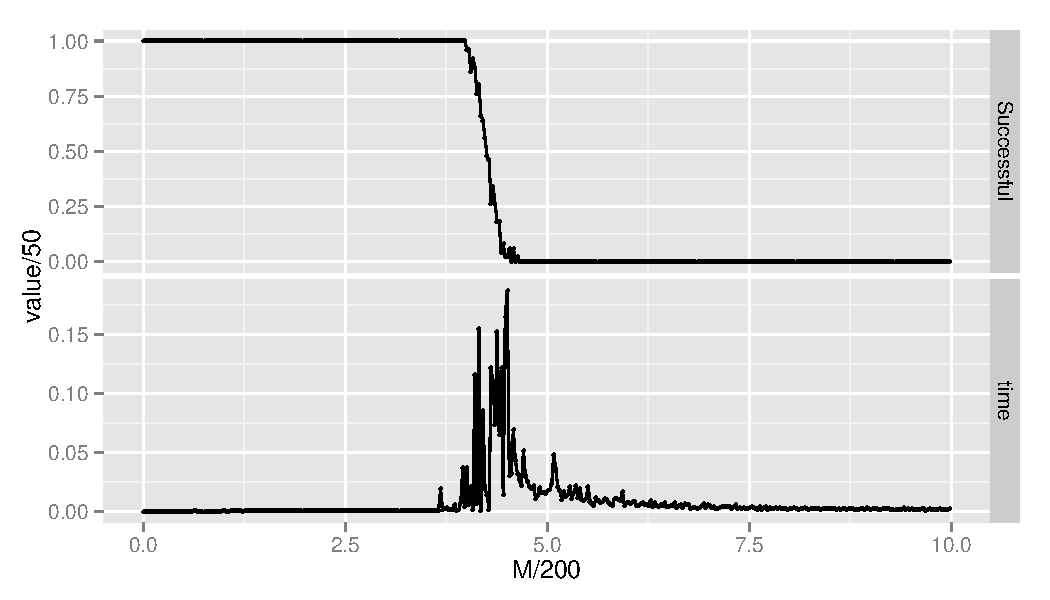
\includegraphics[width=.8\textwidth]{../material_2/plot_sat.pdf}
\caption{Loesungsfindungsdauer von 3SAT-Instanzen mit 1000 Klauseln für ver- schiedene Anzahl von Variablen.} \label{fig:distr}
\end{figure}

Das K -Erfüllbarkeitsproblem (im Folgenden\emph{ KSAT} genannt) gehört zur Klasse der NP-Vollständigen Probleme. KSAT ist, für K > 3, ein zentrales Problem in der kombinatorischen Optimierung und war das erste Problem, für das die NP-Vollständigkeit gezeigt werden konnte \cite{mezard2002random}.

Problembeschreibung: K - Erfüllbarkeitsproblem (nach  \cite{mezard2002random})
Gegeben sei eine Menge $\mathcal{B}$, bestehend aus N booleschen Variablen. Aus dieser Menge $\mathcal{B}$ werden dann K Variablen ausgewählt. Die ausgewählten Variablen, oder deren Verneinungen, werden dann durch (K-1) Oder-Operatoren zu einer \emph {Klausel} zusammengefasst. Auf diese Art und Weise werden M Klauseln gebildet. Durch anwenden von (M-1) Und - Operatoren entsteht so eine KSAT-Instanz.\\Das KSAT-Problem ist nun die Frage, ob eine Belegung der boolschen Variablen aus $\mathcal{B}$ existiert, so dass eine gegebene KSAT-Instanz erfüllbar ist.

In dieser Arbeit werden ausschließlich zufällig generierte KSAT-Instanzen für K=3 betrachtet. Diese Probleme werden dann 3SAT genannt und sind nach \cite{cook1971complexity} NP-Vollständing.

\subsection{Kritischer Punkt bei zufällig generierten KSAT-Instanzen}\label{krit:sat}
Bei zufällig generierten KSAT-Instanen kann beobachtet werden, die Wahrscheinlichkeit, eine korrekte Lösung für die Instanz zu finden, abrupt sinkt, wenn ein kritischer Wert $\alpha_{c}$ (gebildet aus dem Verhältnis von Anzahl der Klauseln zu Anzahl der Variablen) überschritten wird \cite{monasson1996entropy}.

Nach \cite{mezard2002random} liegt dieser kritische Punkt bei zufällig erzeugten 3SAT-Instanzen bei \\$\alpha_{c} \approx 4,267$. In der Umgebung des kritschen Punkts ist die Lösungsfindung (damit ist hier nicht nur eine konkrete Belegung gemeint, falls die Instanz lösbar ist, sondern auch die Erkenntnis, dass diese Instanz nicht gelöst werden kann) algorithmisch komplex. Abb. \ref{crit_sat} verdeutlicht dieses Phänomen visuell.

Zur Erstellung von Abb. \ref{crit_sat} wurden mit Hilfe des \emph{Tough SAT Generators}\footnote{https://toughsat.appspot.com/} 3SAT-Instanzen zu je 1000 Klauseln erstellt. Die Größe der  Menge der boolschen Variablen wurde ausgehend von 1000 schrittweise um 10 verringert, bis ein abschließendes Klausel zu Variablenverhältnis von ca. 7 erreicht wurde. Für jede Größe der so erzeugten Variablenmenge wurden 10 Instanzen erzeugt. Die verschiedenen Instanzen wurden dann mit dem SAT-Solver \emph{Minisat}\footnote{http://minisat.se/} gelöst. In Abb. \ref{crit_sat} ist dann einmal die durchschnittliche sowie die maximale Lösungsdauer der 10 Instanzen für ein bestimmtes Verhältnis dargestellt.
 %%%%%%%%%%%%%%%%% Maximum-Weight Independetn Set %%%%%%%%%%%%%%%%%%%%%%%%%%%%%%%%%%%%%%%%%%%%
%\subsection{Das Problem der maximal gewichteten unabhängigen Menge}\label{chap:wmis}
%
%--Unabhängige Menge \cite{feo1994greedy}]\label{def:unabhmenge}
%Gegeben sei ein Graph $\mathcal{G} = (V,E)$, wobei V die Menge der Knoten des Graphs ist und E die Menge der Kanten des Graphs.\\Eine \emph{unabhängige Menge} von $\mathcal{G}$ ist eine Menge V' $\subset$ V mit folgender Eigenschaft:
%\begin{equation}
%(i,j) \notin E \;\;\;\forall i,j \in V' 
%\end{equation}
%Eine \emph{unabhänginge Menge} eines Graphen $\mathcal{G}$ ist also eine Teilmenge V' der Knoten von $\mathcal{G}$ so, dass die Knoten aus V' paarweise nicht direkt durch eine Kante von $\mathcal{G}$  verbunden sind.
%
%--Maximal gewichtete unabhängige Menge \cite{choi2010adiabatic}
%Gegeben sei ein ungerichteter Graph $\mathcal{G} = (V, E)$, wobei V die Menge der Knoten und E die Menge der Kanten von $\mathcal{G}$ sind, bei dem jeder Knoten v $\in$ V mit einem positiven reellen Gewicht $c_{v}$ versehen wird.\\
%Das Problem ist es dann eine Menge S $\subset$ V zu finden, so dass S eine unabhängige Menge im Sinne von Def. \ref{def:unabhmenge} ist und das Gesamtgewicht von S, gegeben durch $\sum_{v \in S} c_{v}$, maximal ist. Die optimale Lösung wird auch mit WMIS($\mathcal{G}$ ) bezeichnet.
%
%\noindent
%Das Problem der maximal gewichteten unabhängingen Menge wird im Folgenden \emph{WMIS} (engl. Weighted Maximum Independent Set) genannt. Für dieses Problem existiert die folgende QUBO-Darstellung:
%
%Es sei der gleiche Graph $\mathcal{G}$ wie aus der vorhergehenden Problembeschreibung gegeben. Die QUBO-Formulierung des WMIS-Problems lautet dann:
%\begin{equation}\label{wmis:qubo}
%Maximiere \;\;\mathcal{Y}(x_{1},...,x_{n}) = \sum_{i \in V}c_{i}x_{i} - \sum_{i,j \in E}J_{ij}x_{i}x_{j}
%\end{equation}
%
%
%Ist in gerade definierter QUBO-Darstellung des WMIS-Problems $J_{ij} > min \{c_{i},c_{j}\}$ für alle i,j $\in$ E dann ist das WMIS von $\mathcal{G}$ gegeben durch $WMIS(\mathcal{G})=\{v \in V: x^*_{v}=1\}$, wobei $(x^*_{1},...,x^*_{n})$ = arg $max_{(x_{1},...x_{n})\in{0,1}^n} \mathcal{Y}(x_{1},...,x_{n}).$
%
%Es sei  $(x^*_{1},...,x^*_{n})$ = arg $max_{(x_{1},...x_{n})\in{0,1}^n} \mathcal{Y}(x_{1},...,x_{n})$. Weiter sei S* = $\{v \in V: x^*_{v}=1\}$ gegeben. Angenommen, S* ist keine unabhängige Menge. Es gibt also zwei Knoten x,y $\in$ S* die durch eine Kante aus $\mathcal{G}$ verbunden sind. Ohne Beschränkung der Allgemeinheit kann angenommen werden, dass $c_{x} < c_{y}$ gilt. Als nächstes entfernt man x aus S* und bezeichnet mit S' = S*\textbackslash\{x\} die so entstandene Menge. Das Gewicht von S' unterscheidet sich dann durch das Gewicht von S* durch den Ausdruck $-c_{x} + \sum_{j \in nbr(y) \cap S^*}J_{ij} > -c_{y} + J_{yz} > 0$, mit nbr(y) = $\{ z \in V: (z,y) \in E\}$. Das bedeutet also S' hat ein größeres Gewicht als S*, was einen Widerspruch zur Optimalität von S* darstellt. Die Annahme muss also falsch gewesen sein und S* muss eine unabhängige Menge sein. 
